\hsection{Integers}%
\label{sec:int}%
%
Integer arithmetic is the very first thing that you learn in mathematics in primary school.
Integer arithmetic is also the very first thing you learn here.
\emph{Integer} is a Latin word that means \inQuotes{whole} or \inQuotes{intact.}
The integers include all whole numbers and negative numbers and zero, without fractions and decimals.

In many programming languages, there are different integer datatypes with different ranges.
In \pgls{Java}, a \pythonil{byte} is an integer datatype with range~\intRange{-2^7}{2^7-1}, a \pythonil{short} has range~\intRange{-2^{15}}{2^{17}-1}, an \pythonilIdx{int} has range~\intRange{-2^{31}}{2^{31}-1}, and \pythonil{long} has range~\intRange{-2^{63}}{2^{63}-1}, for example.
The draft for the \softwareStyle{C17} standard for the \pgls{C}~programming language lists five signed and five unsigned integer types, plus several ways to extend them~\cite{ISOIEC98892017PLCWDOS}.
The different integer types of both languages have different ranges and sizes, and the programmer must carefully choose which she needs to use in which situation.

\python~3 only has one integer type, called \pythonilIdx{int}.
This type has basically an unbounded range.
The \python~3 interpreter will allocate as much memory as is needed to store the number you want.\footnote{%
Ok, the range is not actually \emph{unbounded}, it is bounded by the amount of memory available on your computer{\dots} {\dots}but for all intents and purposes within this book, we can assume that~$\pythonilIdx{int}\equiv\integerNumbers$.}%
%
\hsection{Integer Arithmetics}%
\label{sec:int:integerArithmetics}%
Now, what can we do with integer numbers?
We can add, subtract, multiply, divide, \glsdisp{modulodiv}{modulo divide}, and raise them to powers, for example.

\begin{figure}%
\centering%
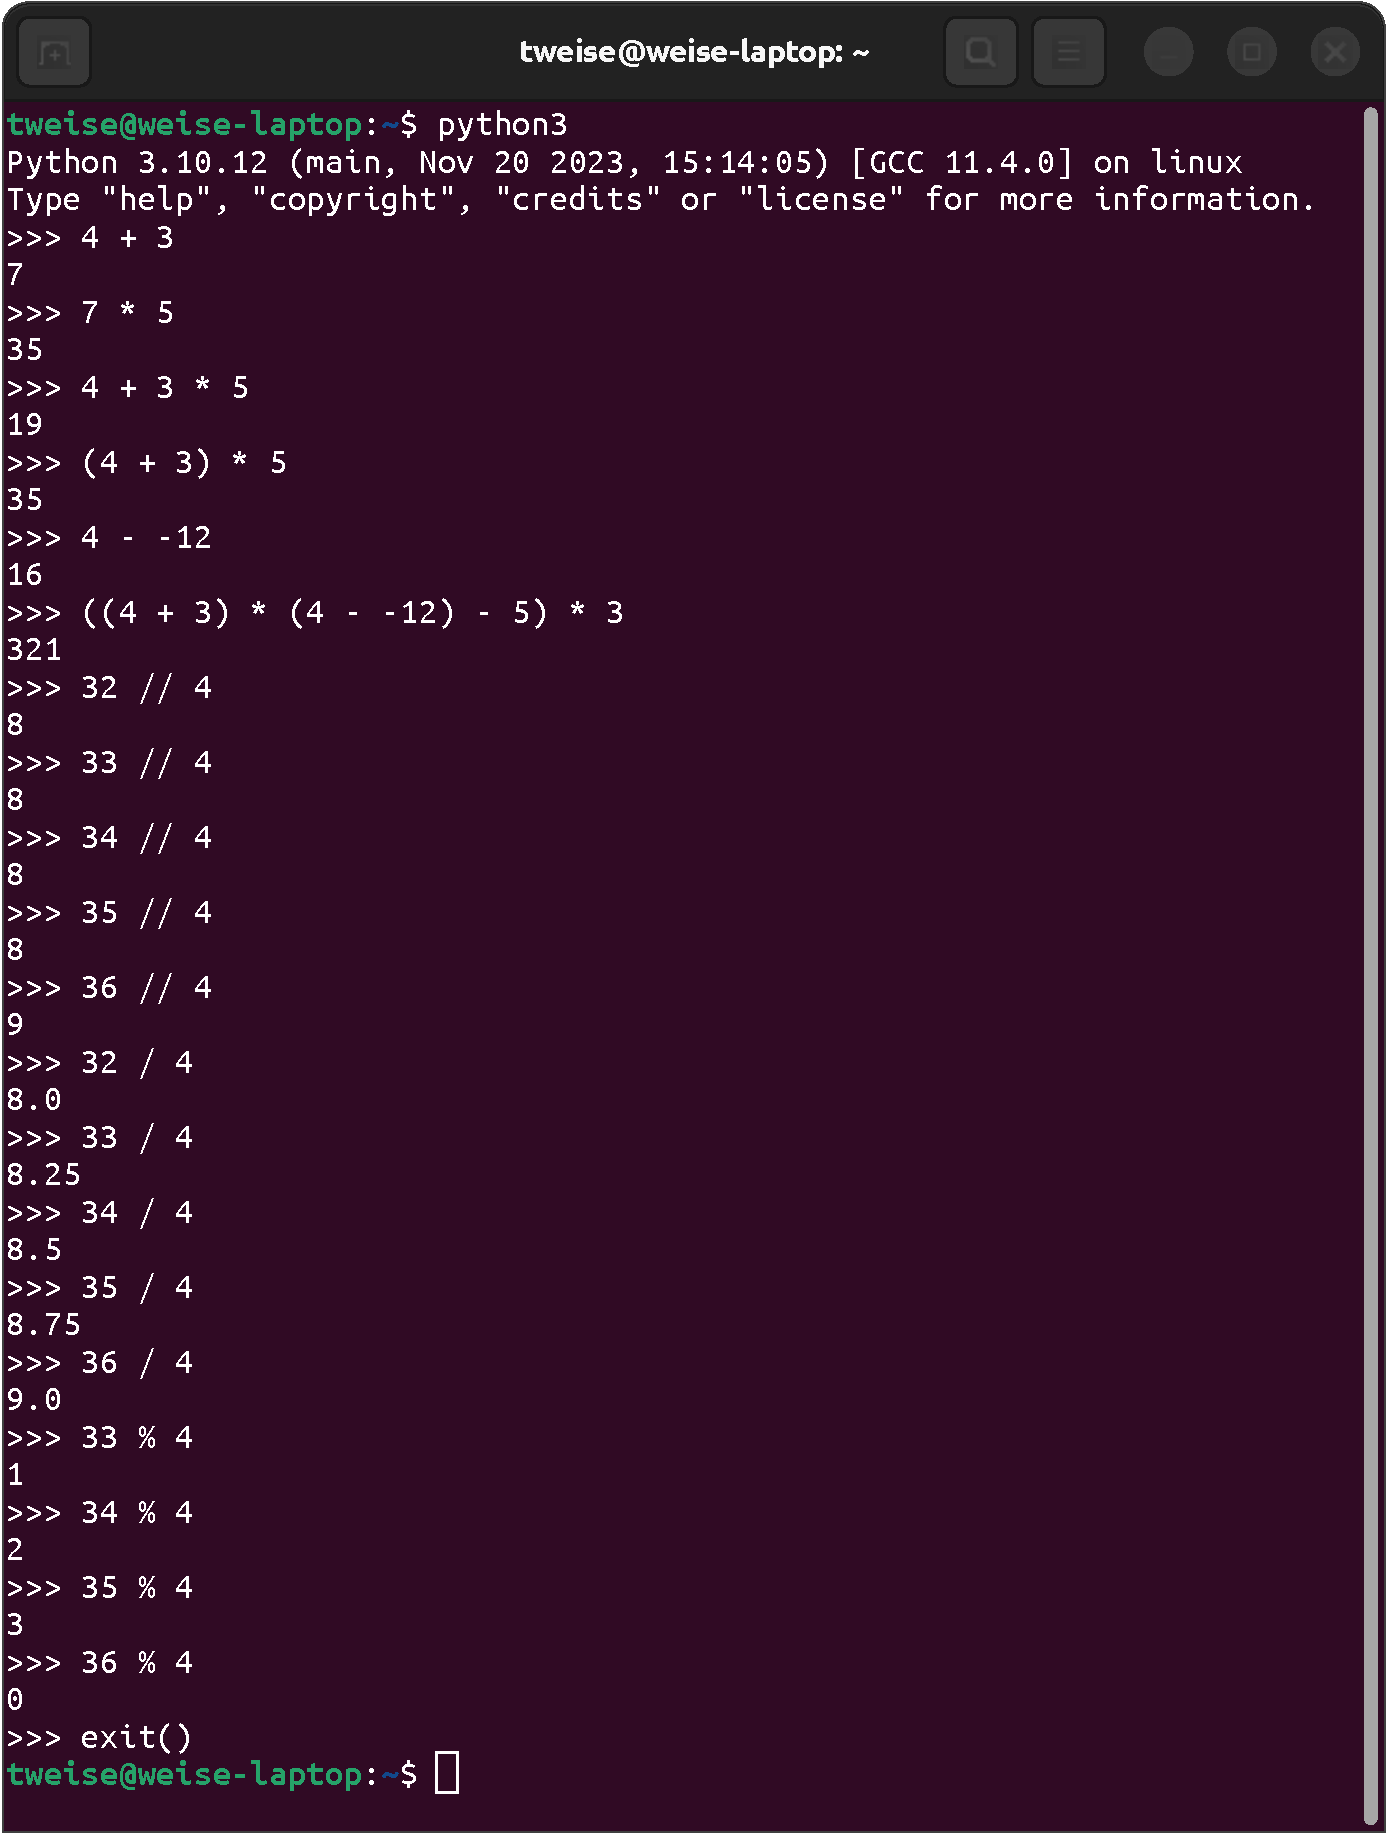
\includegraphics[width=0.8\linewidth]{\currentDir/pythonIntMathInConsoleArith}%
\caption{Examples of \python\ integer math in the console, part~1 (see \cref{exec:int_arithmetics} for part~2).}%
\label{fig:pythonIntMathInConsoleArith}%
\end{figure}%
%
\gitEvalPython{int_arithmetics}{}{simple_datatypes/int_arithmetics.py}%
\listingBox{exec:int_arithmetics}{The same examples of \python\ integer math in the \python\ console as given in \cref{fig:pythonIntMathInConsoleArith}, just as listing instead of screenshot.}{,style=python_console_style}%

In \cref{fig:pythonIntMathInConsoleArith}, you can find some examples of this.
(The same example is given in \cref{exec:int_arithmetics}, just as listing instead of screenshot.
We will use such listings from now on, as they convey the exactly same information, but are easier to read and I can more conveniently include comments.)
Like back in \cref{sec:terminalConsolem}, press \ubuntuTerminal\ under \ubuntu\ \linux\ or \windowsTerminal\ under \microsoftWindows\ to open a \pgls{terminal}.
After entering \bashil{python3} and hitting \keys{\enter}, we can begin experimenting with integer maths.
The lines with \python\ commands in the console begin with \pythonil{>>>}, whereas the result is directly output below them without prefix string.

In the very first line of \cref{fig:pythonIntMathInConsoleArith,exec:int_arithmetics}, we enter \pythonil{4 + 3}\pythonIdx{+} and hit \keys{\enter}.
The result is displayed on the next line and, as expected, is \pythonil{7}.
We then attempt to multiply the two integers \pythonil{7} and \pythonil{5} by typing \pythonil{7 * 5}\pythonIdx{*!multiplication} and hitting \keys{\enter}.
The result is \pythonil{35}.

\python\ does not just support normal arithmetics as you have learned it in school, it also follows the operator precedence rules.
If we type in \pythonil{4 + 3 * 5}, it will compute $4+(3*5)=4+15=19$\pythonIdx{(}\pythonIdx{)} and, hence, print~\pythonil{19}.
We can also use parentheses and type in \pythonil{(4 + 3) * 5}, which will be evaluated as, well $(4+3)*5=7*5=35$, and we get \pythonil{35}.
Integers can be signed, so typing \pythonil{4 - -12}\pythonIdx{-} yields~\python{16}.
Parentheses can be arbitrarily nested, so we can also compute \pythonil{((4 + 3) * (4 - -12) - 5) * 3}, which evaluates to $((7 * 16) - 5) * 3 = (112-5)*3=107*3=321$\pythonIdx{(}\pythonIdx{)}.

Division is a bit tricky in programming in general and in \python\ as well.
There are \emph{two kinds} of division in \python: Integer division, denoted by \pythonilIdx{//} and fractional division, denoted as \pythonilIdx{/}.

\pythonil{32 // 4} yields \pythonil{8}, because \pythonil{4} fits \pythonil{8} times into~\pythonil{32}.
\pythonil{33 // 4}, \pythonil{34 // 4}, and \pythonil{35 // 4} all still yield~\pythonil{8}, as \pythonil{4} \emph{completely} fits \pythonil{8} times into these numbers (leaving some remainder left over).
\pythonil{36 // 4} then finally yields~\pythonil{9}.
The results of the integer division operator \pythonilIdx{//} are always also \pythonils{int}\pythonIdx{int}.

Fractional division, however, returns \pythonilIdx{float} values, which we will explore in the next section (\cref{sec:float}) in detail.
For now, let's just say that they can represent fractional parts (to a limited precision), which is denoted by having a \python{.} in the text output of the numbers.
Computing \pythonil{32 / 4} thus yields~\pythonil{8.0}, \pythonil{33 / 4} gives us \pythonil{8.25}, \pythonil{34 / 4} yields~\pythonil{8.5}, \pythonil{35 / 4} results in \pythonil{8.75}, and, finally, \pythonil{36 / 4} returns~\pythonil{9.0}.
Notice that the result of this division operator is always a floating point number, even if the number itself is an integer.

\bestPractice{intDivision}{Always be careful with which division operator you use for \pythonils{int}\pythonIdx{int}. %
If you need an integer result, make sure to use \pythonilIdx{//}. %
Remember that \pythonilIdx{/} always returns a \pythonilIdx{float} (and see \cref{bp:floatImprecise}), even if the result is a whole number.}

Now above we have said that \pythonil{33 // 4} yields the integer~\pythonil{8}.
The remainder of this operation can be computed using the \pgls{modulodiv} operator \expandafter\pythonilIdx{\%}, i.e., by typing \pythonil{33 \% 4}, which yields~\pythonil{1}.
We also find that \expandafter\pythonil{34 \% 4} yields~\pythonil{2}, \expandafter\pythonil{35 \% 4} gives us~\pythonil{3}, and \expandafter\pythonil{36 \% 4} is~\pythonil{0}.

\gitEvalPython{int_powers}{}{simple_datatypes/int_powers.py}%
\listingBox{exec:int_powers}{Examples of \python\ integer math (powers) in the \python\ console, part~2 (see \cref{exec:int_arithmetics} for part~1).}{,style=python_console_style,literate={0}{0\-}1 {1}{1\-}1 {2}{2\-}1 {3}{3\-}1 {4}{4\-}1 {5}{5\-}1 {6}{6\-}1 {7}{7\-}1 {8}{8\-}1 {9}{9\-}1,breakatwhitespace=false,breaklines=true}

As you will find in \cref{exec:int_arithmetics}, integers can also be raised to a power.
For example, $2^7$~is expressed as \pythonil{2 ** 7}\pythonIdx{**!power} in \python\ (and yields~\pythonil{128}).
\pythonil{7 ** 11}, i.e., $7^{11}$ gives us~1\decSep977\decSep326\decSep743 and shows as \pythonil{1977326743} in the output.

In many programming languages such as \pgls{Java} and \pgls{C}, the largest integer type available off the shelf is 64~bits wide.
If it is signed (can have negative values) like \pgls{Java}'s \pythonil{long}, it has range~\intRange{-2^{63}}{2^{63}-1}.
An unsinged 64~bit integer type, such as \pythonil{unsigned long long} in \pgls{C}, would have range~\intRange{0}{2^{64}-1}.
In \python\, we can compute $2^{63}$~(\pythonil{2 ** 63}), namely 9\decSep223\decSep372\decSep036\decSep854\decSep775\decSep808, and
$2^{64}$~(\pythonil{2 ** 64}), which is~18\decSep446\decSep744\decSep073\decSep709\decSep551\decSep616.
These are very large numbers and the latter one would overflow the range of the standard integer types of \pgls{Java} and \pgls{C}.
However, we can also keep going and compute \pythonil{2 ** 1024}, which is such a huge number that it wraps several times in the output of our \python\ console in \cref{exec:int_arithmetics}!
\python\ integers are basically unbounded~(or bounded only by the memory size of our computer).
However, the larger they get, the more memory they need and the longer it will take to compute with them.
\endhsection%
%
\hsection{Operations on Bit Strings}%
\label{sec:int:bitstrings}%
%
\noviceHint{%
You are encouraged to skip over this section.
This section is about integers numbers from the perspective of bit strings and the bit string based operations that we can apply to them.
If you are learning programming, then this part is not important now.
You can circle back to it later.}%
%
\begin{figure}%
\centering%
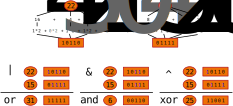
\includegraphics[width=0.8\linewidth]{\currentDir/binaryMath}%
\caption{Examples for how integer numbers are represented as bit strings in the computer (upper part) and for the binary (bitwise) operations \emph{and}, \emph{or}, and \emph{exclusive or} (often called~\emph{xor}).}%
\label{fig:binaryMath}%
\end{figure}
\gitEvalPython{int_binary}{}{simple_datatypes/int_binary.py}%
\listingBox{exec:int_binary}{Examples of the binary representation of integers and the operations that apply to it.}{,style=python_console_style}

All integer numbers can be represented as bit strings.
In other words, a number $z\in\integerNumbers$ can be expressed as $b_0 2^0 + b_1 2^1 + b_2 2^2 + b_3 2^3 + b_4 2^4\dots$, where the $b_i$-values each are either~0 or~1.
Then, $\dots b_4 b_3 b_2 b_1 b_0$ is a bit string.
If we represent integers with such strings of five bits, then the number~1 would have representation~\texttt{00001}, because it is equivalent to~$2^0$.
In in \cref{fig:binaryMath}, we illustrate that the number~22 would be \texttt{10110} because $22=2^4+2^2+2^1$ and the number~15 would correspond to \texttt{01111}, as~$15=2^3+2^2+2^1+2^0$.

We can obtain the binary representation of integer numbers as text using the \pythonilIdx{bin} function in \python.
As shown in \cref{exec:int_binary}, \pythonil{bin(22)} yields \pythonil{'0b10110'}.
Here, the \pythonilIdx{0b} prefix means that the following number is in binary representation.
We can also enter numbers in binary representation in the console.
Typing \pythonil{0b10110} corresponds to the number~\pythonil{22}.
Similarly, \pythonil{bin(15)} yields \pythonil{'0b1111'} and entering \pythonil{0b1111} into the console corresponds to entering the number~\pythonil{15}.

In \python, we can compute the bitwise (i.e., binary) \emph{or}, \emph{and}, as well as the and \emph{exclusive~or} of this binary representation of integers using the \pythonil{|}, \pythonil{&}, and \pythonil{^} operators, respectively.
Binary \emph{or} returns an integer in which all bits are set to~1 which were~1 in either of its two operands.
\pythonil{22 | 1}\pythonIdx{\textbar!bit-wise or} yields \pythonil{23}, because the bit with value~1 is not set in~22 and the binary~\emph{or} sets it (effectively adding~1 to~22).
The slightly more comprehensive example \pythonil{22 | 15} sketched in \cref{fig:binaryMath} gives us \pythonil{31}, because $22=2^4+2^2+2^1$ and $15=2^3+2^2+2^1+2^0$, which \pythonil{|} combines to $31=2^4+2^3+2^2+2^1+2^0$, i.e., each power of~2 that occurred in either of the two operands is present in the result.
\pythonil{bin(31)} yields \pythonil{'0b11111'}.

Binary \emph{and} returns the integer where only the bits remain~1 that were~1 in \emph{both} operands.
Applying binary \emph{and} instead of \emph{or}, i.e., doing \pythonil{22 & 1}\pythonIdx{\&} results in~\pythonil{0}, because, as said before, the bit $2^0$ is not set in~22.
\pythonil{22 & 15}, yields~\pythonil{6}, because only $2^2$ and $2^1$ appear both in~22 and~15.
Thus, \pythonil{bin(6)} corresponds to \pythonil{'0b110'}.

The \emph{exclusive~or}, which is often called \emph{xor}, will set a bit to~1 if it is~1 in exactly one of the two operands.
Therefore, \pythonil{22 ^ 1}\pythonIdx{\^{}} gives~\pythonil{23}, since only the bit with value $2^0$ is set in~1 and the other bits that are~1 in~22 are not.
\pythonil{22 ^ 15} yields \pythonil{25}, because $2^4$, $2^3$, and $2^0$ occur only once in the two operators (whereas $2^2$ and $2^1$ occured in both of them).
This is confirmed by typing \pythonil{bin(25)}, which results in \pythonil{'0b11001'}.

Finally, we can also shift bit strings to the left or right by $i$~places.
The former corresponds to multiplying with~$2^i$, the latter is the same as an integer division by~$2^i$.
Shifting \pythonil{22} by one bit position to the \emph{left} -- which is done by entering \pythonil{22 << 1}\pythonIdx{<\strut<} -- therefore results in~\pythonil{44}.
We already know that \pythonil{bin(22)} is \pythonil{'0b10110'} and so it comes at no surprise that \pythonil{bin(44)} is \pythonil{'0b101100'} (notice the additional \pythonil{0} that appeared on the right hand side).
Shifting \pythonil{22} by two bit positions to the \emph{right} -- which is done by entering \pythonil{22 >> 2}\pythonIdx{>\strut>} -- results in \pythonil{5}.
The \pythonil{10} on the right hand side of the binary representation disappeared, as \pythonil{bin(5)} is \pythonil{'0b101'}.

Besides the binary representation of integer numbers, which is to the basis~2, there also exists the hexadecimal representation (base~16) and the octal representation (base~7).
We can obtain the hexadecimal representation of~22 by computing \pythonil{hex(22)}\pythonIdx{hex} and get \pythonil{0x16}\pythonIdx{0x}, which corresponds to~$1*16^1+6*1=22$.
We can also enter hexadecimal numbers in the console like \pythonil{0x16}, which yields~\pythonil{22}.
The octal representation of~22 is obtained as \pythonil{oct(22)}\pythonIdx{oct}, which produces \pythonil{0o26}\pythonIdx{0o}, which, in turn, corresponds to~$2*8^1+6$.
Similarly, this octal number can be entered as \pythonil{0o26}.
With this, our excursion into binary maths ends and we now welcome back all first-time readers.%
%
\endhsection%
%
\hsection{Summary}%
In conclusion, the integer type \pythonilIdx{int} represents whole numbers.
Integers can be positive or negative or zero.
All the primitive mathematical operations like addition, subtraction, multiplication, and division that you learned in school can be applied to integers.
The normal arithmetic precedence rules (that you also have learned in school) apply.
Parentheses can be used to group operations.
Finally, \python\ also provides the same binary logic operators, working on the bit string representation of integers, that you may or or may not know from other programming languages as well.
\endhsection%
\FloatBarrier%
\endhsection%
%
